
% modeling Dominion in Hakaru, and what kinds of questions are interesting
% to ask the model
\section{Case Study: Dominion} \label{sec:dom}

Dominion is a game we are familiar with. This game is known as a turn-based
deckbuilding game, where a player \emph{builds} a good deck by choosing what
cards to buy on their turn. The probabilistic component of deckbuilding games
arises from shuffling decks of cards at certain points in the game. In particular
in Dominion the cards a player plays can affect both when cards get shuffled
and the composition of the deck being shuffled. As a result, game-play heuristics
for Dominion are inherently intertwined with the probabilistic game state.

\subsection{Game State}

\subsection{Heuristics} \label{sec:dom:heuristics}
We

\subsection{Greedy Results}
We present results for the greedy heuristic just described in
Section \ref{sec:dom:heuristics}. The simplest query one might wish to ask of
the greedy heuristic is:

\begin{quote} \label{quote:dominion-query}
Given that we buy card $X$ with probability $p0$ and card $Y$ with
probability $(1 - p0)$, what is the distribution over the length of
the game?
\end{quote}

In this query, we have model parameters of:

\begin{itemize}
\item $X$  \mintinline{haskell}{:: Card}
\item $Y$  \mintinline{haskell}{:: Card}
\item $p0$ \mintinline{haskell}{:: Probability}
\end{itemize}

\begin{figure}
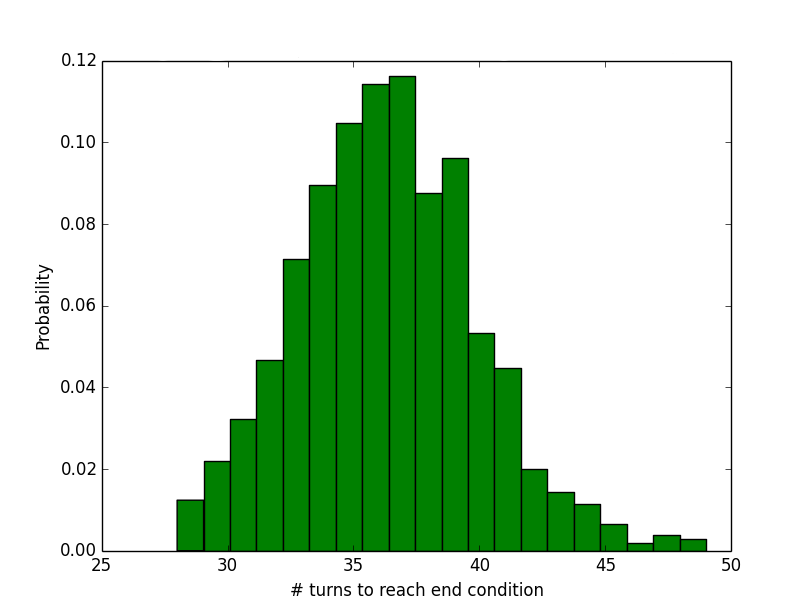
\includegraphics[width=.95\columnwidth]{../pres/village-chancellor-turn-dist.png}
\caption{\label{fig:turn-dist} Probability distribution over number of turns
in a 2-player game of Dominion.
Both players play a greedy strategy with model
parameters of $X = \textrm{Village}$, $Y = \textrm{Chancellor}$, and
$p_0 = 0.5$. See Appendix \ref{app:dominion-card} for a complete description
of the semantics behind these cards and why this pair of cards is interesting
for the game Dominion.
This distributions is unconditioned, therefore only requiring sampling directly
from the model (no inference).
}\end{figure}

One observe-query inference question to ask the model then is:

\begin{equation} \label{eqn-inference-question}
...
\end{equation}

